\chapter{Introduction}

\section{Qu'est-ce que GénialBall ?}

GénialBall est un jeu de sport, dans un mélange de football et d’air-hockey, où deux joueurs s’affrontent en réseau local, ayant comme but de pousser le ballon dans le but adverse.\\

\section{Comment y jouer ?}

Lancez l'application, choississez d'être le client ou le serveur ( un joueur doit être le client, l'autre doit être le serveur), attendez que la recherche d'IP local se termine, puis selectionnez l'IP local de votre adversaire.
%inclusion d'une mage dans le document
\begin{figure}[!h]
\begin{center}
%taille de l'image en largeur
%remplacer "width" par "height" pour régler la hauteur
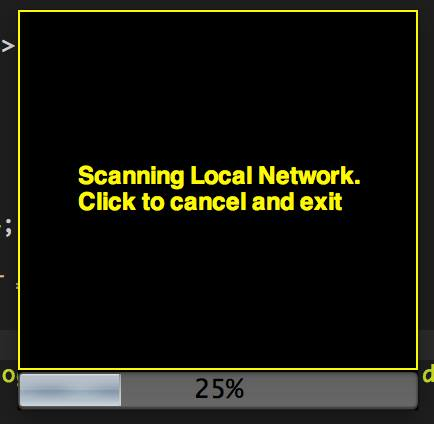
\includegraphics[width=5cm]{./ScanningNetwork}
%légende de l'image
\caption{Le jeu va d'abord chercher les autres machines connectées dans le réseau local.}
\end{center}
\end{figure}

\begin{figure}[!h]
\begin{center}
%taille de l'image en largeur
%remplacer "width" par "height" pour régler la hauteur
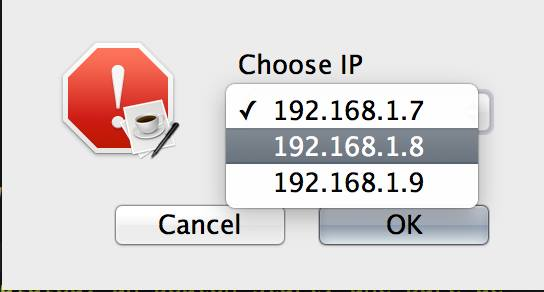
\includegraphics[width=5cm]{./ChooseYourIp}
%légende de l'image
\caption{Sélectionnez ensuite l'IP local de votre adversaire}
\end{center}
\end{figure}

\newpage

\section{Interface du jeu}
%inclusion d'une mage dans le document
\begin{figure}[!h]
\begin{center}
%taille de l'image en largeur
%remplacer "width" par "height" pour régler la hauteur
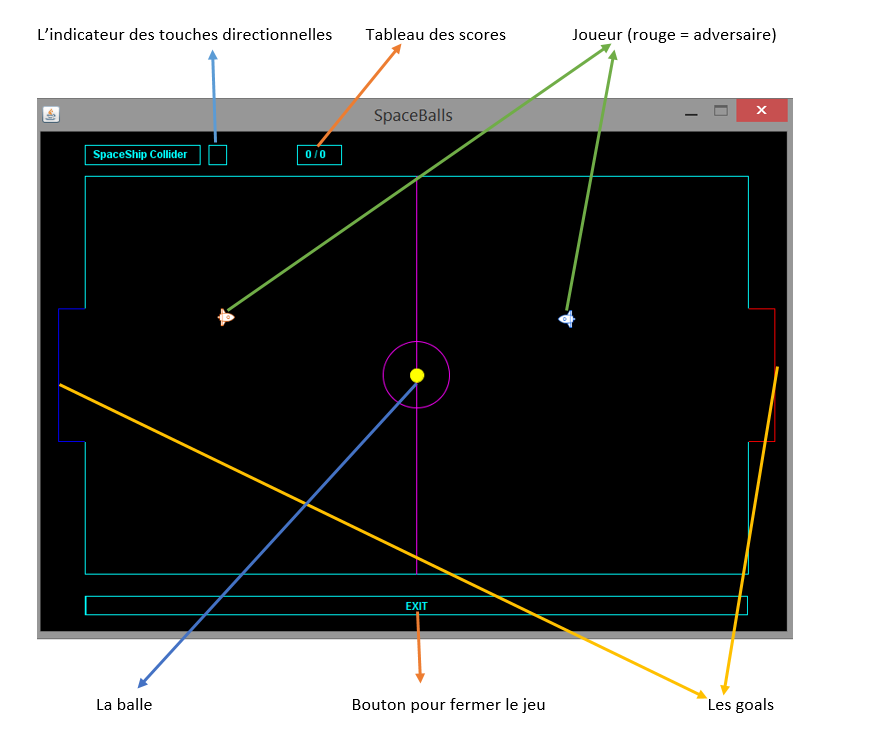
\includegraphics[width=20cm]{./InterfaceGraph}
\end{center}
\end{figure}

\section {Les contrôles du jeu}

\begin{itemize}
\item Utilisez les touches directionnelles pour déplacer votre vaisseau.
\item Appuyez sur la barre d'espace si vous désirez faire un tir avec la balle.
\item Si vous désirez quitter, cliquez sur la touche "Exit" ou appuyez sur Esc.
\end{itemize}

